%% This is file `elsarticle-template-1-num.tex',
%%
%% Copyright 2009 Elsevier Ltd
%%
%% This file is part of the 'Elsarticle Bundle'.
%% ---------------------------------------------
%%
%% It may be distributed under the conditions of the LaTeX Project Public
%% License, either version 1.2 of this license or (at your option) any
%% later version.  The latest version of this license is in
%%    http://www.latex-project.org/lppl.txt
%% and version 1.2 or later is part of all distributions of LaTeX
%% version 1999/12/01 or later.
%%
%% Template article for Elsevier's document class `elsarticle'
%% with numbered style bibliographic references
%%
%% $Id: elsarticle-template-1-num.tex 149 2009-10-08 05:01:15Z rishi $
%% $URL: http://lenova.river-valley.com/svn/elsbst/trunk/elsarticle-template-1-num.tex $
%%
\documentclass[preprint,12pt]{elsarticle}
% \documentclass[preprint,12pt]{article}

%% Use the option review to obtain double line spacing
%% \documentclass[preprint,review,12pt]{elsarticle}

%% Use the options 1p,twocolumn; 3p; 3p,twocolumn; 5p; or 5p,twocolumn
%% for a journal layout:
%% \documentclass[final,1p,times]{elsarticle}
%% \documentclass[final,1p,times,twocolumn]{elsarticle}
%% \documentclass[final,3p,times]{elsarticle}
%% \documentclass[final,3p,times,twocolumn]{elsarticle}
%% \documentclass[final,5p,times]{elsarticle}
%% \documentclass[final,5p,times,twocolumn]{elsarticle}

%% The graphicx package provides the includegraphics command.
\usepackage{graphicx}
%% The amssymb package provides various useful mathematical symbols
\usepackage{amssymb}
%% The amsthm package provides extended theorem environments
%% \usepackage{amsthm}

\usepackage{authblk}

\usepackage{hyperref}

\usepackage{biblatex}

\addbibresource{references.bib}


\journal{Lancet Public Health}

\begin{document}
\begin{frontmatter}

\title{Maximizing education while minimizing risk: a model-based analysis of reopening schools during a COVID-19 pandemic}


%\author[add1]{Jamie A. Cohen}
%\author[add1]{Dina Mistry}
%\author[add1,add2]{Cliff C. Kerr}
%\author[add1]{Daniel J. Klein}
%\ead{dklein@idmod.org}

%\address[add1]{Institute for Disease Modeling, Seattle, WA, USA}
%\address[add2]{University of Sydney, Sydney, NSW, Australia}


% \begin{document}

\begin{abstract}
%% Text of abstract
To be written.
\end{abstract}

\begin{keyword}
COVID-19 \sep Agent-based modeling \sep Disease transmission
%% keywords here, in the form: keyword \sep keyword

%% MSC codes here, in the form: \MSC code \sep code
%% or \MSC[2008] code \sep code (2000 is the default)

\end{keyword}

% \maketitle
\end{frontmatter}

%% \listoffigures

%% \linenumbers

\section{Introduction}

Public K-12 schools around the country and world closed due to COVID-19 transmission in March and April of 2020. A recent study has estimated that school closures were associated with a significant decline in both COVID-19 incidence and mortality \cite{auger_association_2020}. 

Attention is now focused on the risks and benefits of reopening schools. The educational, social, and physical benefits of in-person learning are enormous; they provide a safe space for educational instruction, support the development of social and emotional skills, and address nutritional needs. For these reasons and more, the American Academy of Pediatrics issued a statement \cite{AAPstatement} on July 10 advocating for bringing students back to the classroom for in-person learning. 

Yet much remains uncertain about the role schools, and school-age students in particular, play in COVID-19 transmission, as well as how effective school-based interventions will be in preventing transmission. While children may be both less susceptible and less likely to develop severe infection, nearly a quarter of teachers are at a greater risk of serious illness if infected with COVID-19 \cite{claxton_how_2020}. In an NPR/Ipsos poll of 505 teachers across the US conducted in July, 77 percent of teachers indicated that they are worried about risking their own health in returning to in-person education and 66 percent would prefer primarily remote, distance learning \cite{kamenetz_most_2020}.

Much can be learned from the experience of school reopening across Europe and Asia; many countries successfully reopened without a significant increase in COVID-19 cases, while others were forced to quickly re-close after outbreaks were observed in multiple schools \cite{vegas_reopening_2020, couzin-frankel_school_2020}. In general, countries that reopened schools tended to do so when the case detection rate over the most recent 14 day period was below 25 per 100,000 -- nearly 10 times lower than the case detection rate in the United States as of August 11 (NEED A CITE), with significant heterogeneity both across and within states. Additionally, many of these settings returned younger students in-person first with some degree of staggering the start, stop, and break times within schools.

In this analysis, we used an agent-based model of COVID-19 transmission to %estimate the impact of school closures on transmission within schools and the community and to % 
evaluate the health and educational outcomes associated with various school reopening strategies. Specifically we compared behavioral interventions such as mask usage, physical distancing and hand hygiene; case detection interventions, including symptomatic screening, follow-up diagnostic testing and contact tracing; and structural interventions, including classroom cohorting, schedule changes, and combinations of remote and in-person learning. %We also compare strategies for reactive classroom and school closure following the detection of a COVID-19 case in school.

\section{Methods}
\subsection{Model overview}
We used Covasim, an agent-based model of COVID-19 transmission and interventions \cite{kerr_controlling_2020, kerr_covasim_2020}, to estimate the impact of school reopening on disease transmission and the extent to which school-based interventions could mitigate epidemic spread within and outside schools. Covasim includes demographic information on age structure and population size; realistic transmission networks in different social layers, including households, schools, workplaces, long-term care facilities and communities; age-specific disease outcomes; and within- and between-host variations in infectivity to capture sub- and super-spreading and front-loaded infectivity. We modeled schools to match age mixing patterns between students within elementary schools, middle schools, and high schools \cite{guclu_social_2016} (see \hyperref[sec:AppendixA]{Appendix A} for more details on the school network structures). Key inputs and assumptions of our modeling approach have been documented in our methodology papers \cite{kerr_controlling_2020, kerr_covasim_2020}.

\subsection{Calibration}

We fit the model to the directional trend and size of the COVID-19 epidemic and use data from King County, Washington to define the population distribution and network structure. We used the effective reproductive number in the absence of school reopening and the case detection rate in the two weeks prior to school reopening as signals of both the direction of cases as well as the size of the epidemic (see \hyperref[sec:AppendixB]{Appendix B} for details on calibration).The results we present reflect the case where the epidemic is declining slowly when schools are fully closed (i.e., R\textsubscript{e} = 0.9). In conjunction with our assumption around epidemic growth or control with full school closures, we considered three scenarios for the size of the epidemic in the two weeks prior to school reopening: 20, 50, or 110 cases per 100,000 individuals. These numbers were chosen to fit within the low ($<$25), medium (25 - 75) and high ($>$75) case detection bands defined by the Washington State Department of Health that tie reopening recommendations to epidemic metrics (CITE DOH decision tree). %We simulated a test positivity rate of approximately 2-3\%, but did not vary this as part of the analysis. 

\subsection{Analytic methodology}

We identified and compared seven alternative school reopening strategies:
\begin{enumerate}
    \item All in person with no countermeasures
    \item All in person with countermeasures
    \item All in person with countermeasures and A/B scheduling
    \item Elementary and middle in person with countermeasures, high school remote
    \item Elementary in person with countermeasures, middle and high school remote
    \item Elementary in person with countermeasures and A/B scheduling, middle and high school remote
    \item All remote
\end{enumerate}

Countermeasures are non-pharmaceutical interventions (NPIs), which implicitly include face masks, six foot separation, and hand washing, which together are assumed to reduce transmission by 25\%; class cohorting, in which students and teachers have no contact outside their own classroom; and symptomatic screening, with 50\% follow-up diagnostic testing and 50\% follow-up contact tracing. A/B scheduling splits classrooms into group A students (who attend two days per week, e.g. Mon-Tue) and group B (who attend two different days per week, e.g. Thu-Fri).

We applied our interventions to elementary, middle, and high schools and assumed that pre-schools and universities will remain closed. We assumed that high schools would not be able to implement classroom cohorting, as it would be too challenging to coordinate the highly variable schedules of students at this level. We simulated the first three months of the school term (Sept. 1\textsuperscript{st} - Dec. 1\textsuperscript{st}).

\section{Results}

In-person schooling, even with sufficient countermeasures, poses significant risks to students, teachers, and staff. Even on the first day of school, we find that 5\% - 42\% of schools would have at least one person arrive at school with active COVID-19 (including all students, teachers, and staff), depending on the incidence of COVID in the community and the school type (Figure \ref{fig:schools_with_a_case}). These infections may show few symptoms and go undetected, especially if they are in younger children. Symptomatic individuals may stay home or be screened and sent home immediately upon arrival. Active COVID-19 infections also may not lead to onward transmission within schools, depending on per-contact infectivity. This highlights the importance of procedures within schools to minimize risk of transmission, detect and isolate cases, and contact and quarantine any known contacts. 

\begin{figure}[h]
    \centering
    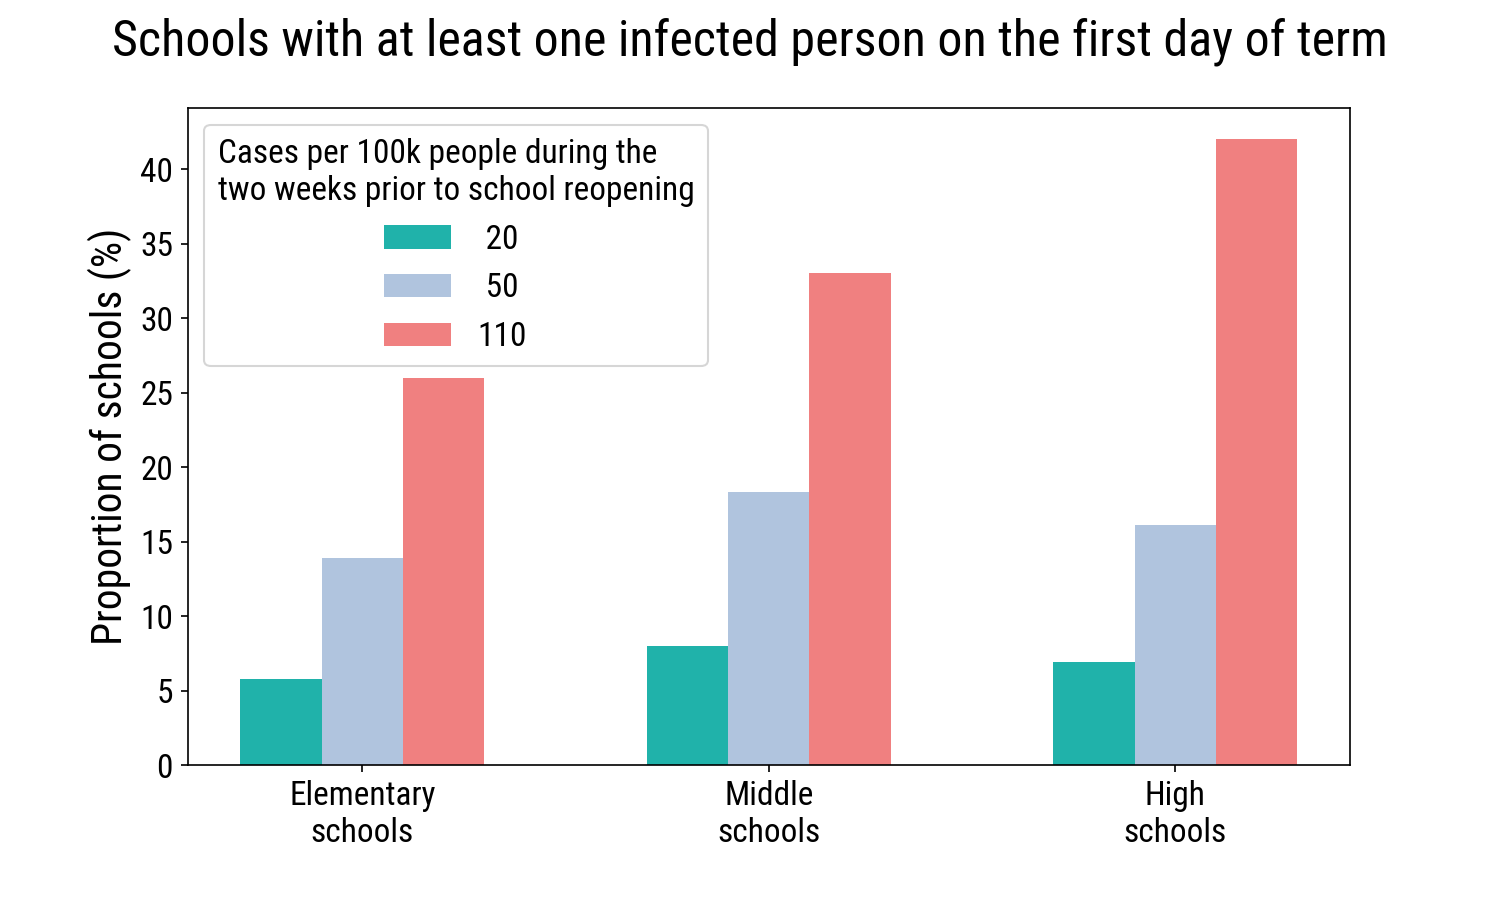
\includegraphics[scale=0.5]{schools_with_a_case_2020-08-05.png}
    \caption{Percent of schools with at least one infectious individual on the first day of school, averaged across the top 20 parameter sets.}
    \label{fig:schools_with_a_case}
\end{figure}

Closely examining infections present in school, our model shows that either A/B school scheduling or an incremental approach that returns elementary schools in person and keeps all other students remote can mitigate the presence of COVID within (and outside of) schools. In the absence of any countermeasures in schools, we can expect between 6 and 25 percent of teaching and non-teaching staff and between 4 and 20 percent of students to be infected with COVID in the first three months of school, depending upon the incidence rate (Figure \ref{fig:attack_rate}): when there is more COVID in the population, there will inevitably be more COVID in schools. Schools can lower this risk to as low as 0.2 percent for staff and 0.1 percent for students by returning elementary schools with a hybrid schedule while all other grades continue learning remotely. We estimate that this approach would require an additional 900 - 6,200 tests for students, teachers and staff over the first three months of school, depending on the case detection rate in the two weeks prior to school.

\begin{figure}[h]
    \centering
    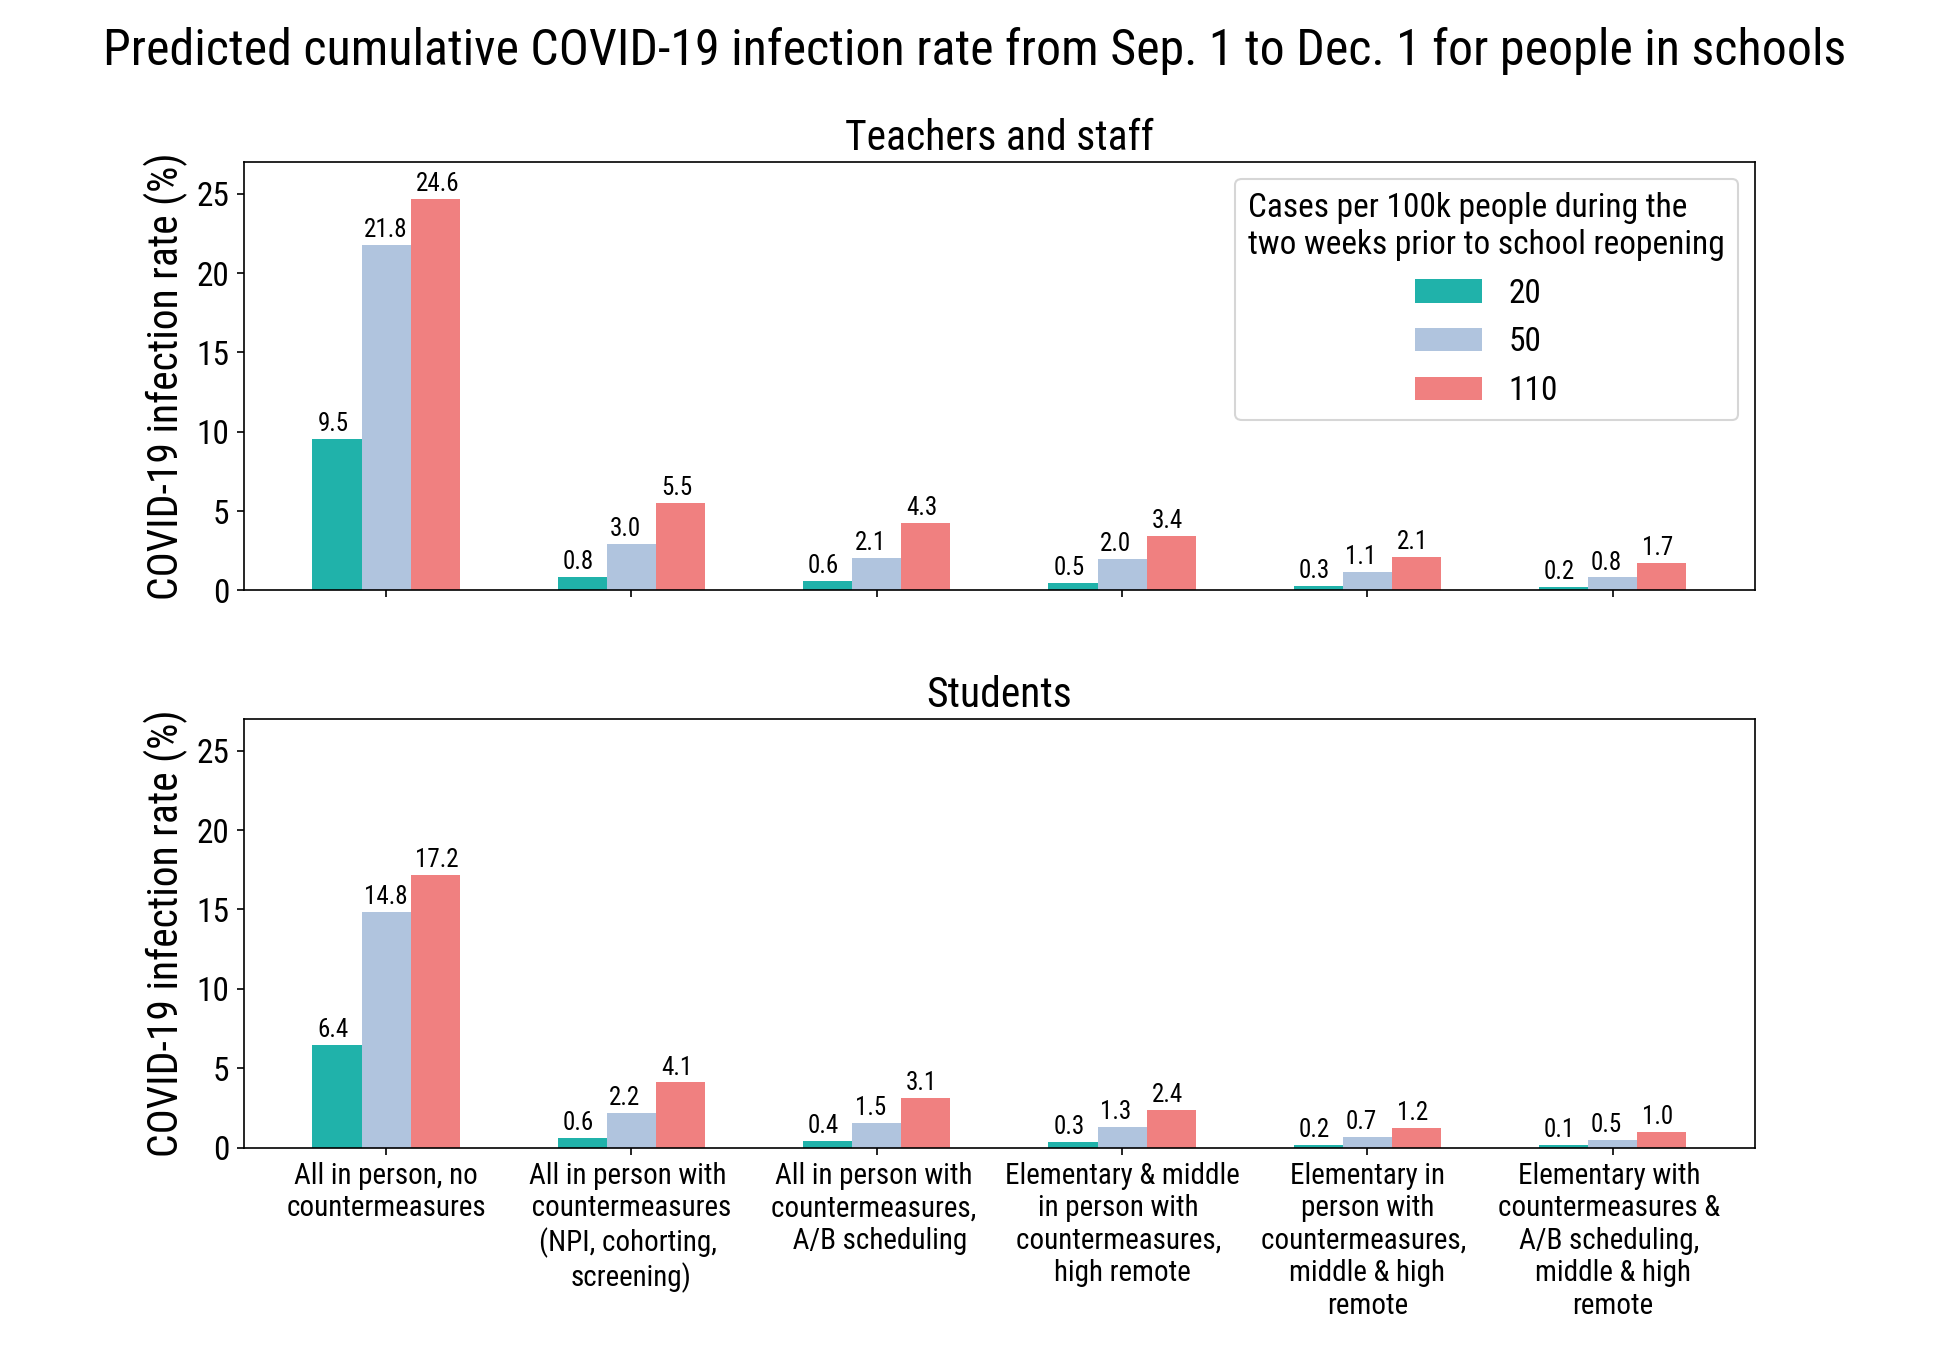
\includegraphics[scale=0.4]{attack_rate_2020-08-06.png}
    \caption{Cumulative COVID-19 infection rate for students, teachers and staff physically present in schools during the period of school reopening (Sept 1\textsuperscript{st} - Dec 1\textsuperscript{st}), averaged across the top 20 parameter sets.}
    \label{fig:attack_rate}
\end{figure}

We find that an A/B scheduling approach, in which classrooms are split into two groups that attend school two days a week on different days, reduces COVID-19 transmission in schools nearly as much as an elementary only approach. The key difference between these approaches is that A/B scheduling gives all K-12 students some time for in-person learning, whereas the elementary-only approach restricts in-person learning to elementary school students, at least initially.

These strategies come at a significant educational cost, requiring up to 83 percent of school days to be spent at home, due to either planned distance learning or related to detected COVID-19 infection (Figure \ref{fig:tradeoffs}). We find that, provided sufficient countermeasures within schools, the COVID-19 infection rate in the population prior to school reopening has more influence on the COVID-19 infection rate within schools than the specific reopening strategy: we expect an over seven times reduction in the infection rate for people in schools if schools are reopened when the incidence rate in the community is at 20 per 100,000 compared to 110 per 100,000. At any given size of community transmission, additional countermeasures will have a much more marginal impact on the rate of infection within schools for a large cost of missed in-person school days. We note that days of distance learning are not experienced equally by students and the benefit gained varies considerably based on both age and other factors such as socioeconomic status and resources available to their families.

\begin{figure}[h]
    \centering
    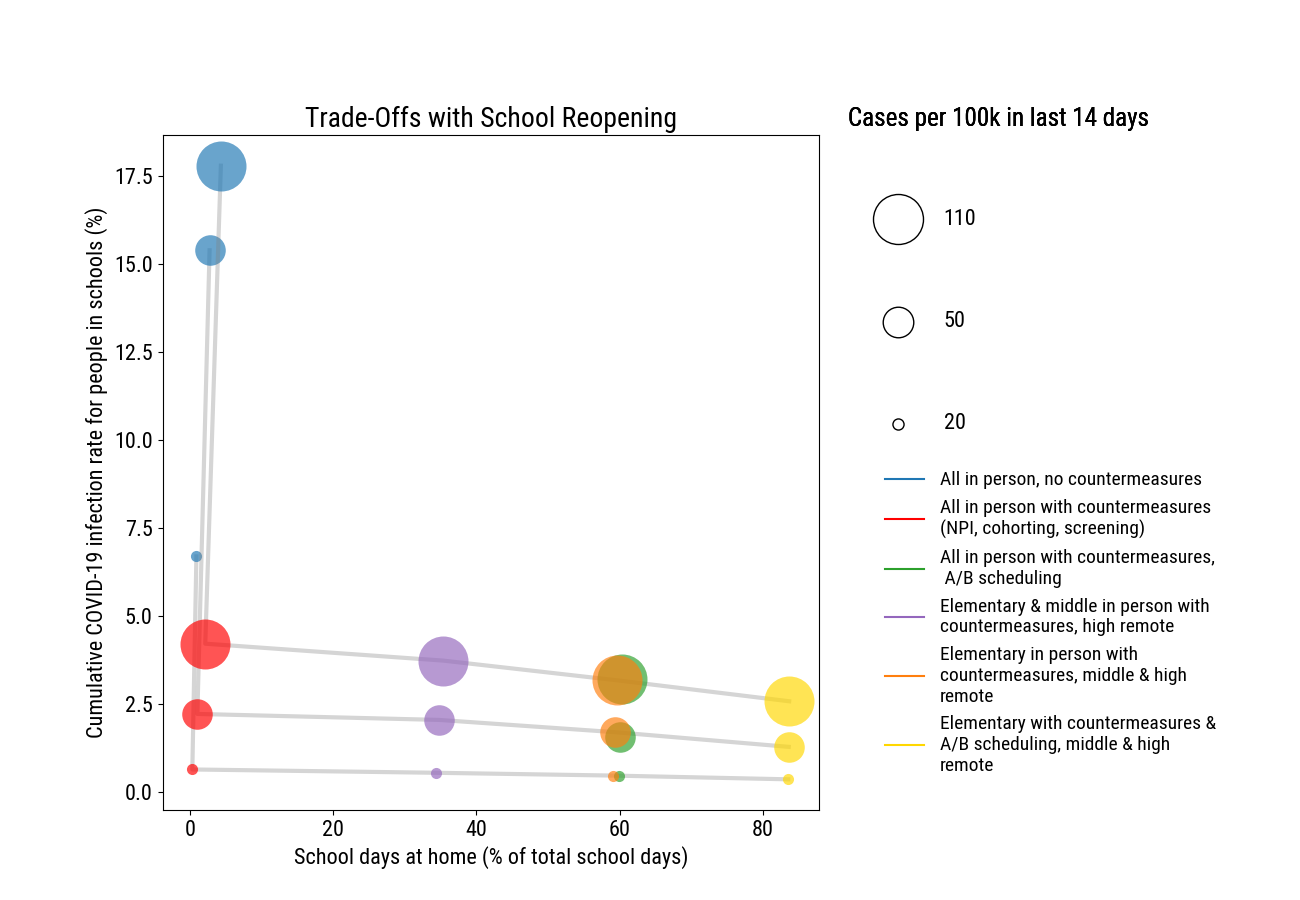
\includegraphics[scale=0.48]{tradeoffs_2020-08-06.png}
    \caption{Trade-offs between within-school infection rate and missed in-person school days (due to either scheduled distance learning, quarantine or infection.}
    \label{fig:tradeoffs}
\end{figure}

We find that reopening schools will not significantly increase community-wide transmission, provided sufficient school-based interventions are implemented (Figure \ref{fig:reff}). If community transmission is decreasing in the absence of in-person schooling, we can return to in-person learning with appropriate countermeasures without adding to community transmission. 

\begin{figure}[h]
    \centering
    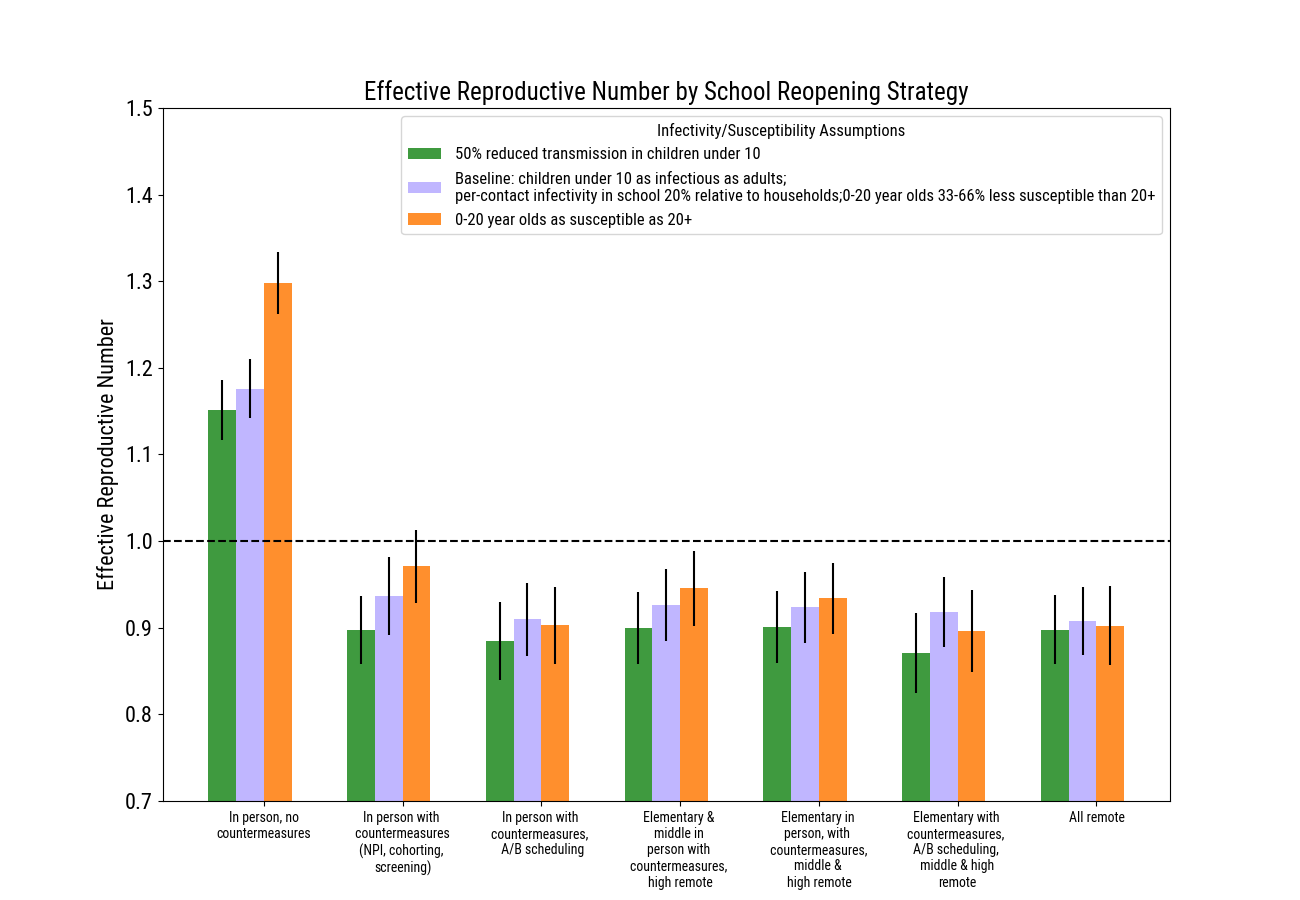
\includegraphics[scale=0.4]{r_eff_2020-08-13.png}
    \caption{Effective reproductive number over the simulated period of school reopening (Sept 1\textsuperscript{st} - Dec 1\textsuperscript{st}) averaged across the top 20 parameter sets, assuming a COVID-19 incidence rate of 50 cases per 100,000 in the 14 days prior to school reopening. Error bars represent the standard deviation of the top 20 parameter sets.}
    \label{fig:reff}
\end{figure}

\subsection{Sensitivity analysis}

Due to considerable uncertainty in the roles K-12 students, teachers, and staff play in COVID-19 transmission, we performed several sensitivity analyses to see if results were robust to a range of reasonable assumptions. A recent study using data from South Korea suggests that students under the age of 10 might be half as infectious as older students and adults \cite{park_early_nodate}. Implementing this variation in the model only further supports the elementary-only approach. Our results are robust when we reduced the infectivity of children under 10 years old by 50 percent (Figure \ref{fig:attack_rate_sens}).

\begin{figure}[h]
    \centering
    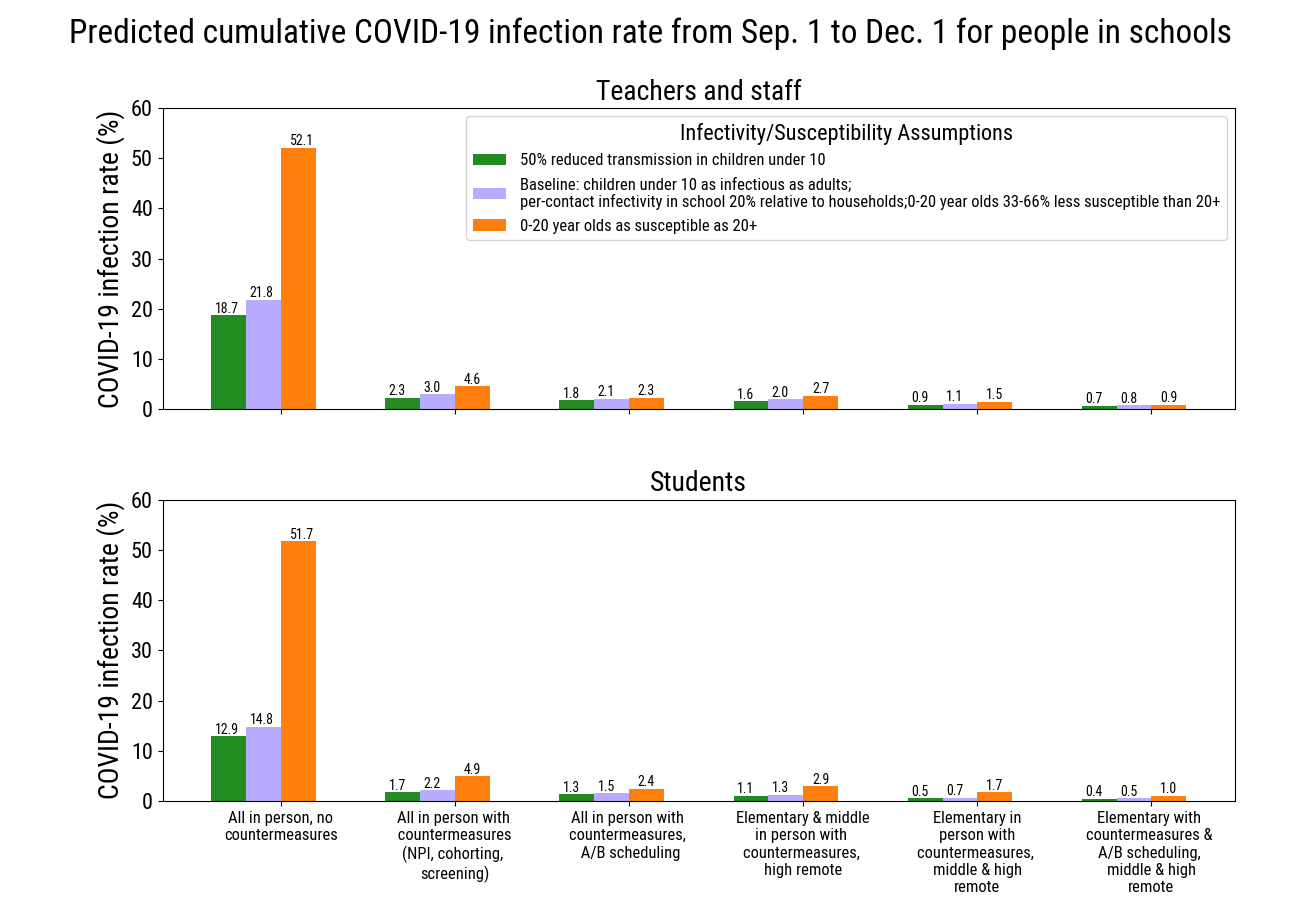
\includegraphics[scale=0.4]{attack_rate_sens_2020-08-13.png}
    \caption{Cumulative COVID-19 infection rate for students, teachers and staff physically present in schools during the period of school reopening (Sept 1\textsuperscript{st} - Dec 1\textsuperscript{st}), averaged across the top 20 parameter sets, assuming a COVID-19 incidence rate of 50 cases per 100,000 in the 14 days prior to school reopening.}
    \label{fig:attack_rate_sens}
\end{figure}

A second sensitivity analysis concerns the susceptibility of school-age children to COVID-19 infection. In our base case, we assume that 0-10 year-olds have a 66 percent reduced susceptibility to infection and 10-20 year-olds have a 33 percent reduced susceptibility to infection \cite{zhang_changes_2020}. However, a recent study among children in Australia challenges this broadly held assumption, arguing that children are similarly vulnerable and transmit the virus to a meaningful degree \cite{hyde_covid-19_2020}. We find that without any countermeasures in schools, this assumption has a significant impact on the infection rate for people in schools (Figure \ref{fig:attack_rate_sens}) as well as the effective reproductive number in the community (Figure \ref{fig:reff}). With sufficient countermeasures, this assumption does not seem to change our general policy conclusions.


\section{Discussion}

Return to in-person learning will pose significant risks for students, staff and teachers. However, our results suggest that, depending on the incidence of COVID-19 in the community, a carefully organized incremental approach that returns the youngest students first with a reduced schedule would minimize the risk of infection within schools and provide important benefits to the neediest children. While this analysis is based upon school enrollment and population demographic data from King County, Washington, lessons can be applied to other settings to inform decision-making around school reopening. For example, as of August 11, 2020, Seattle had a 14-day case detection rate of 150 compared to 50 in New York City per 100,000 people. Our modeling suggests this would translate to nearly twice as many schools in Seattle with at least one person arriving at school with an active COVID-19 infection on September 1\textsuperscript{st} compared to New York City, depending on the size of the school. It may also indicate a different optimal strategy for school reopening in these cities. In fact, Seattle Public Schools, citing a case detection rate in the city of well over 75 per 100,000 in the last two weeks, announced they would be starting the fall with completely remote learning, while New York Public Schools announced they would start with an A/B hybrid scheduling approach \cite{zaveri_new_2020}.

We find that the solution with the lowest health risk also has the highest educational cost, the majority of which lands on those communities and families already most under-resourced: those without access to technology and whose parents are essential workers. Decision makers must therefore balance the benefits of in-person education with the safety of teachers and staff, while continuing efforts to decrease the incidence of COVID-19 outside of schools. Regardless of the approach taken, it will be critical to monitor schools with symptomatic screening and react quickly to the emergence of cases in schools with testing and contact tracing.

Our results support the strategy of returning elementary school students to school either full-time or with an A/B schedule while keeping all other students remote for the first three months of school to best minimize the risk of COVID-19 infection in schools. Returning elementary schools in-person first is both relatively lower-risk and higher-benefit—elementary school aged children are less susceptible to infection \cite{zhang_changes_2020} and potentially less likely to transmit infection \cite{park_early_nodate}. Additionally, they benefit more from in-person learning and pose more of a burden on family members. These results can be supported by experience globally, where we have seen countries return elementary school aged students to school and returning older students at a later stage after observing an absence of significant school-based transmission \cite{zhang_changes_2020, auger_association_2020}. However, these countries had a significantly lower COVID-19 incidence rate prior to reopening schools than many parts of the country, including Washington State, are experiencing today.

\subsection{Limitations}

While agent-based modeling is able to capture many details of populations and disease transmission, our work has important limitations and assumptions that could impact our findings. There is still a high degree of uncertainty around the susceptibility, symptomiticity/severity, and infectivity of COVID-19 in children, particularly since schools in most locations shut down early in the epidemic. Our analysis is based on the most recent scientific literature for each of these parameters. We assumed individuals under 20 had a 45-50\% reduced risk of developing symptoms \cite{davies_age-dependent_nodate} and 33-66\% reduced risk of acquiring infection \cite{zhang_changes_2020}. We varied this in sensitivity analysis so that individuals under 20 are equally as susceptible to infection as individuals age 20 to 50. We assume that an infectious individual is 5 times more likely per day to transmit to a household contact than a school contact, based on estimated numbers of hours spent in each setting per week. We assume all individuals infected with COVID-19 are equally likely to transmit infection per contact, and varied this assumption in sensitivity analysis so that individuals under 10 years old are half as likely.

After being diagnosed, all individuals are assumed to reduce their daily infectivity by 70\% for home contacts, 90\% for community contacts, and 100\% for school and work contacts. Additionally, the household contacts of these individuals may be traced, notified, and school contacts removed from school for a full 14-day quarantine period. While we anticipate that schools will be able to help identify contacts of diagnosed students or staff, the large number of contacts within schools may place additional burden on local or state contact tracing efforts and our analysis does not represent this. We assume that household transmission is not reduced while children are attending school in person, nor that it increases when students are learning remotely.

In terms of structural choices, we made several assumptions about the implementation and impact of school reopening strategies. We chose to not model increased transmission associated with parents/guardians returning to work following a return to in-person learning. We also assume students who participate in remote learning are not in contact with anyone from school. On days that students are learning remotely, we do not account for any potential interaction students may have in a congregate care setting, such as an alternative after-school care program. We have assumed that, if implemented, all elementary and middle schools will be able to enforce classroom cohorting, whereby students are grouped into a classroom and are only in contact with other students and teachers in that classroom. We note that cohorting may be difficult to implement given the complexity of class scheduling for student bodies with multiple academic tracks, elective classes, and degree requirements. Therefore, we may be underestimating the transmission impact of school reopening, and further caution should be taken in any decisions to return to in-person learning.

We assumed that, if implemented, symptomatic screening would occur daily in schools and students or teachers presenting with COVID-like symptoms would be sent home. Those who are symptomatic may be asked to take a diagnostic test, which we assumed returns a result within two days. Students who received a negative test result return to school the next day, and students who received a positive test result are isolated at home for 14 days. Our results do not depend on school staff administering the diagnostic tests. We are not explicitly modeling after-school care, which many working parents depend upon to cover the gap between school hours and working hours. Families who use these services may also be more likely to be essential workers. We also do not model transportation to and from school, which may be an important source of transmission and which also depends on school resources.


\section{Conclusions}

Schools around the world are grappling with the challenge of returning to in-person learning in the COVID era. Much remains unknown about the role children play in COVID-19 transmission within schools and in the broader community, but the latest science suggests that younger children are less susceptible and show fewer symptoms if infected. From schools that never closed in Sweden to reopening examples in Europe and Asia, lessons on how the US might resume in-person learning are abundant and diverse. Our computational modeling synthesizes this evidence, and the latest results give reason for optimism.

Yet reopening schools is not a zero-risk activity. Symptom screening is imperfect, and COVID-19 will be present in the respiratory system of students, teachers, and staff on day one. Additionally, a return to in-person learning would allow parents and guardians return to work, which could be accompanied by an associated increase in transmission outside schools. But the solution with the lowest health risk has the highest educational cost, the majority of which lands on those families most marginalized and under-resourced: those without access to technology and private tutors, and whose parents or guardians work in the essential economy. Schools must open; the question is when and how, so as to balance the benefits of in-person education with the safety of teachers and staff, all while realizing that COVID is not just a school problem.


\printbibliography

\appendix

\section{Schools network structure}
\label{sec:AppendixA}

We simulated a representative sample of the 2.25 million King County, Washington residents in Covasim. We use student enrollment data for King County available from the 2018 American Community Survey [6]. This data gives an estimate of the enrollment rates by age for students attending any educational institution at the county level. Enrollment rates are given by age groups: 3-4 years old, 5-9 years old, 10-14 years old, 15-17 years old, 18-19 years old, 20-24 years old, 25-34 years old, 35 year old and over. The enrollment rate for the last group is estimated to be less than 3\%   and this rate is applied to ages 35 to 50 years old. School sizes are drawn from a distribution based on the enrollment numbers for Seattle area schools available for the year 2017 [7].

In order to model realistic school reopening scenarios, we equipped the model to generate networks within schools that reflect proposed cohorting by age and grade. We modeled schools to approximate age mixing patterns [3] between students within preschool, elementary schools, middle schools, high schools, and universities.  Using the county-level school enrollment data [6], we simulate contacts within schools, mixing between students and teachers, and clustering of students into cohorts. Mixing of students and teachers can be thought of as following three main patterns: (1) students sorted in classroom cohorts of the same grade with one or two teachers, (2) students mixing with random contacts mostly within the same grade and at least one teacher, and (3) students mixing with random contacts across the entire school and at least one teacher. The first mixing pattern resembles the contact structures commonly found in pre-school and elementary schools, where students are generally taught by one teacher and stay with the same classroom of contacts throughout the day. The second pattern reflects mixing patterns often found in middle schools and high schools where students have individualized schedules and mostly interact with other students in the same grade. The third mixing pattern reflects university settings where student interaction occurs in classes, dorms, and in other spaces on campus. Student mixing in these institutions display less age assortativity because of the high variability of age when students enroll, use of common spaces such as libraries and dining halls, and other aspects of on-campus life. 

In addition to students and teachers, schools also include additional staff members such as principals, counselors, nurses, maintenance, and cleaning staff. Using information on the estimated ratio of students to all staff members, we model the number of additional non teaching staff expected for each school and the contacts for them as random contacts across the entire school. This reflects the overall more varied contact patterns of non-teaching staff with students, teachers, and other staff members.

\section{Calibration}
\label{sec:AppendixB}

We used an optimization procedure to find a set of parameters that resulted in our desired combinations of effective reproductive number in the absence of schools and cumulative incidence in the two weeks prior to the school year. We varied the number of seeded infections at the start of the simulation and the reduction of workplace and community contacts. We ran our analysis with the top 20 best fitting parameter sets (see Table \ref{tab:calibration}).

We calibrated these model parameters using the Tree-structured Parzen Estimator sampler in Optuna, an optimization software. The sampler trains models of $p(\theta|y)$ and $p(y)$, where $\theta$ is a set of parameters and $y$ is a (scalar) output of an objective function, to find the region of the parameter space that minimizes y. We defined the objective function to be the sum of squared differences between observed data (i.e., average effective reproductive number from September 1st to December 1st; cumulative COVID-19 cases in the two weeks prior to September 1st) and the corresponding model predictions. 


\begin{table}[h]
\centering
\begin{tabular}{|c|c|c|}
\hline
\textbf{} & \textbf{\# seeded infections} & \textbf{\% reduction in contacts}\\
\hline
\centering 
20 cases/100k/14d & 81 & 40\% \\
50 cases/100k/14d & 156 & 40\% \\
110 cases/100k/14d & 395 & 43\% \\
\hline
\end{tabular}
\caption{Calibrated Parameter Values (Best fit)}
\label{tab:calibration}
\end{table}



\end{document}

